\chapter{Specyfikacja zewnętrzna}
\label{ch:04}

\section{Wymagania sprzętowe i programowe}

Program wykorzystuje potok programowalny biblioteki OpenGL oraz jednostki cieniujące napisane w~języku GLSL w wersji 3.30. Oznacza to, że~system użytkownika musi posiadać kartę graficzną wspierającą OpenGL co najmniej w~wersji 3.3.
Dodatkowo program wykorzystuje następujące biblioteki, których kod źródłowy znajduje się wewnątrz projektu:
\begin{itemize}
\item GLAD
\item GLFW
\item GLM
\item Dear ImGui
\end{itemize}

Projekt został skompilowany i~przetestowany przy wykorzystaniu kompilatora g++
w~wersji 12.2.0 na~systemie Linux. Kompilacja programu odbywa się przy pomocy narzędzia CMake.

\section{Sposób instalacji}
\subsection{System Linux}
Przykład kompilacji programu został wykonany przy wykorzystaniu systemu Ubuntu 22.04. Pierwszym krokiem jest instalacja narzędzi takich jak program CMake, kompilator języka C i C++, itp. oraz instalacja wymaganych bibliotek.
Do tego celu wykorzystane są następujące polecenia
\begin{figure}[H]
\lstset{basicstyle=\ttfamily, language=bash}
\begin{lstlisting}[language=bash]
  sudo apt install cmake
  sudo apt install build-essential
  sudo apt install xorg-dev
  sudo apt install git
\end{lstlisting}
\end{figure}

Następnym krokiem jest pobranie repozytorium git projektu. Istotnym jest, by pobrać repozytorium rekurencyjnie, gdyż dołączone biblioteki zostały dodane do repozytorium jako submoduły. Można tego dokonać poleceniem
\begin{lstlisting}[language=bash]
  git clone https://github.com/Rei-sen/raymarch-terrain --recursive
\end{lstlisting}
Alternatywnie, jeżeli repozytorium nie zostało pobrane rekurencyjnie, można zastosować polecenia
\begin{lstlisting}[language=bash]
  git submodule init
\end{lstlisting}
a następnie
\begin{lstlisting}[language=bash]
  git submodule update
\end{lstlisting}
Ostatnim krokiem jest wygenerowanie plików reguł Makefile, a następnie
kompilacja projektu. Generacji plików reguł Makefile można dokonać wywołując następujące polecenie w głównym katalogu projektu
\begin{lstlisting}[language=bash]
  cmake -B build -S .
\end{lstlisting}
W celu kompilacji należy wykorzystać poniższe polecenie
\begin{lstlisting}[language=bash]
  cmake --build build
\end{lstlisting}
Końcowy plik wykonywalny o nazwie raymarch-terrain znajduje się w katalogu build.
\subsection{System Windows}
Pierwszym krokiem instalacji programu na systemie Windows jest pobranie
projektu z repozytorium github, które można znaleźć pod adresem
\url{https://github.com/Rei-sen/raymarch-terrain}. Podobnie jak przy instalacji programu na systemie Linux, repozytorium należy pobrać rekurencyjnie, z wszystkimi submodułami.
Dalszą część instalacji można dokonać w~środowisku Visual Studio lub
wykorzystując narzędzie CMake. Oba sposoby zostaną przedstawione poniżej.
\subsubsection{Instalacja przy wykorzystaniu środowiska Visual Studio}
Przed przystąpieniem do otwarcia projektu należy się upewnić, że
wsparcie systemu budowy CMake jest zainstalowane w środowisku Visual Studio.
Można tego dokonać w~instalatorze Visual Studio, jak na rysunku \ref{fig:vs-cmake-install}.

\begin{figure}
\centering
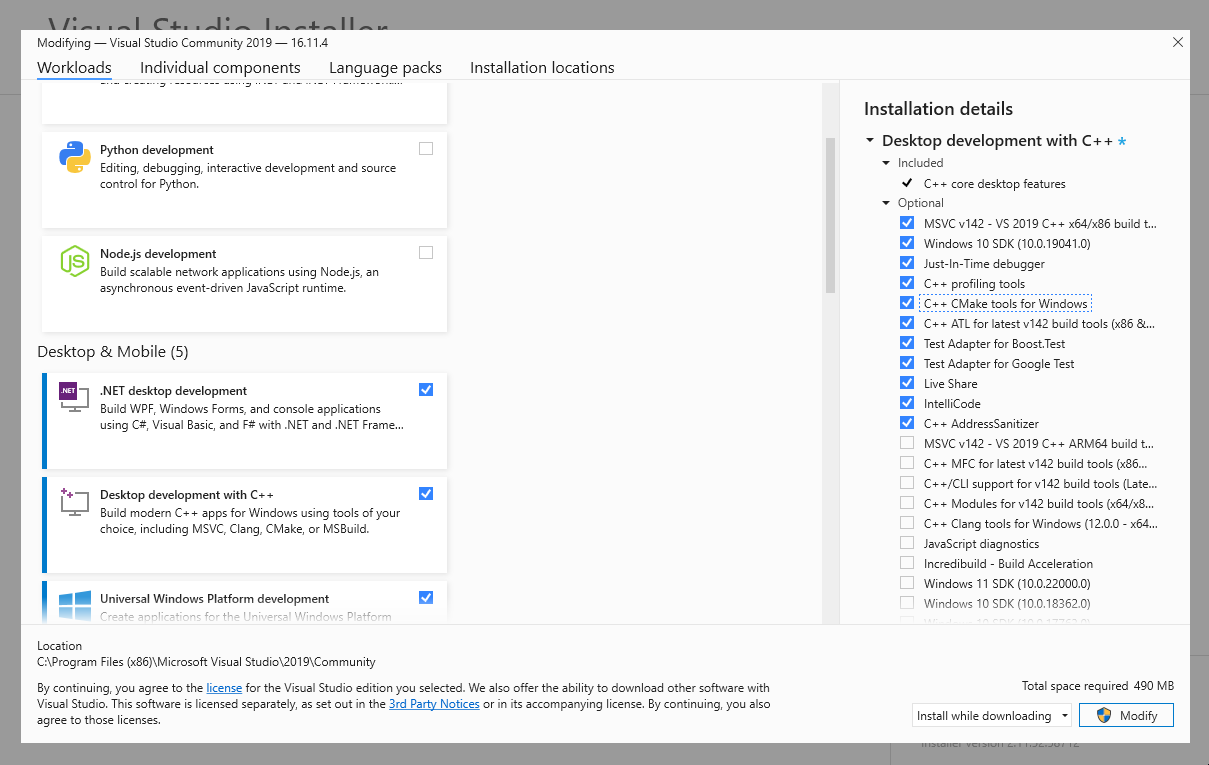
\includegraphics[width=1\textwidth]{./graf/vscmakeinstall.png}
\caption{Instalacja wsparcia systemu CMake w instalatorze środowiska Visual Studio.}
\label{fig:vs-cmake-install}
\end{figure}

Po zweryfikowaniu instalacji wsparcia systemu CMake należy uruchomić środowisko Visual Studio, a następnie wybrać opcję \ang{Open local folder}. Kolejnym krokiem jest wybranie głównego folderu projektu. Po otwarciu projektu i~ukończeniu generacji środowiska CMake, należy zmienić opcję \ang{Select startup item} na raymarcher.exe. Po wykonaniu powyższych kroków, projekt można budować oraz kompilować jak zwykły projekt środowiska Visual Studio.

\subsubsection{Instalacja z wykorzystaniem narzędzia CMake}
Pierwszym etapem jest instalacja narzędzia CMake, które można znaleźć pod adresem \url{https://cmake.org}.
Następnie należy uruchomić narzędzie CMake w trybie graficznym.
Kolejnym etapem jest wybór głównego katalogu projektu oraz katalogu budowy, w którym znajdą się końcowe pliki binarne.
Jako główny katalog projektu należy wskazać katalog, w którym znajduje się plik CMakeLists.txt.
Jako folder budowy został utworzony nowy folder o nazwie \ang{build} w głównym folderze projektu.
Przykład powyższych kroków został przedstawiony na rysunku \ref{fig:cmake-win}.
\begin{figure}[H]
\centering
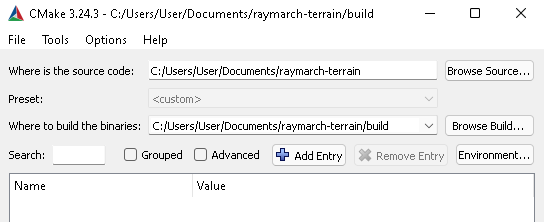
\includegraphics[width=1\textwidth]{./graf/cmake-win.png}
\caption{Wybór folderu projektu oraz folderu budowy narzędziu graficznym CMake.}
\label{fig:cmake-win}
\end{figure}
Kolejnym etapem jest konfiguracja systemu budowy, której można dokonać przyciskiem \ang{Configure}, a następnie wybierając (odpowiednie, interesujące nas) docelowe środowisko programistyczne. Rysunek \ref{fig:cmake-conf} przedstawia przykładową konfigurację dla środowiska Visual Studio 16 dla systemów 64-bitowych.

\begin{figure}[H]
\centering
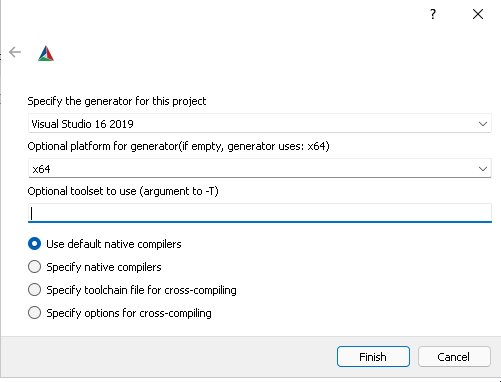
\includegraphics[width=1\textwidth]{./graf/cmake-conf.png}
\caption{Konfiguracja środowiska programistycznego.}
\label{fig:cmake-conf}
\end{figure}

Następnie należy wygenerować pliki budowy, wykorzystując przycisk \ang{Generate}.
Ostatnim etapem jest otwarcie projektu poprzez pliki znajdujące się w folderze budowy lub poprzez przycisk \ang{Open Project} w oknie programu CMake. W dalszej kolejności należy dokonać kompilacji programu, korzystając z wcześniej wybranego środowiska programistycznego.

\section{Sposób obsługi}
Po uruchomieniu program przedstawia prosty interfejs użytkownika, widoczny na~rysunku \ref{fig:ui}. Cały
obszar okna wykorzystywany jest do wyświetlania renderowanego terenu.
Dodatkowo wewnątrz okna renderowany jest obszar zawierający pola
pozwalające na zmianę parametrów związanych z renderowaniem oraz generacją
terenu. Użytkownik ma możliwość poruszania kamerą korzystając z klawiszy W, S, A oraz D. Zmiana orientacji kamery jest możliwa poprzez poruszanie myszką, gdy wciśnięty jest lewy przycisk myszki. Szczegółowe informacje dotyczące korzystania z interfejsu użytkownika można uzyskać naciskając przycisk \ang{Show UI Help}. Program można zakończyć poprzez naciśnięcie przycisku Escape lub zamknięcie okna.

\begin{figure}[H]
\centering
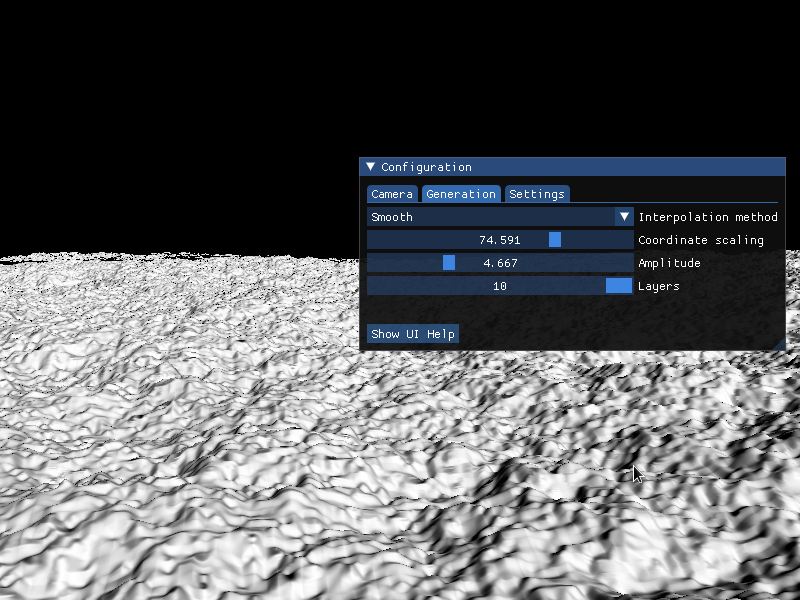
\includegraphics[width=0.95\textwidth]{./graf/ui.png}
\caption{Interfejs użytkownika}
\label{fig:ui}
\end{figure}

\section{Przykład działania}
Program daje użytkownikowi szeroki zakres ustawień związanych z renderowaniem oraz generowaniem terenu. Jedną z takich możliwości jest kontrola ustawień kamery w~zakładce \ang{Camera}, lista dostępnych ustawień:

\begin{itemize}
\item Position - współrzędne, w których znajduje się kamera,
\item FOV - pole widzenia kamery podane w stopniach,
\item Orientation - orientacja kamery:
  \begin{itemize}
    \item Horizontal - obrócenie kamery względem osi Y,podane w radianach,
    \item Vertical - obrócenie kamery względem osi X, podane w radianach.
  \end{itemize}
\end{itemize}

Wygenerowanie pożądanego ukształtowania terenu umożliwione jest przez następujące opcje:

\begin{itemize}
\item Terrain - Ustawienia związane z ukształtowaniem terenu:
  \begin{itemize}
    \item Max terrain rendering steps - maksymalna ilość kroków, renderowania terenu
    \item Interpolation method - Metoda interpolacji wysokości terenu:
      \begin{itemize}
        \item Linear - interpolacja biliniowa,
        \item Smooth - interpolacja z wykorzystaniem funkcji. \ang{smoothstep}
      \end{itemize}
    \item Coordinate scaling - skalowanie współrzędnych X oraz Z,
    \item Amplitude - skalowanie wysokości terenu,
    \item Layers - ilość warstw wykorzystane w technice \ang{fBm},
    \item Layer rotation - Obrócenie współrzędnych punktu dla każdej warstwy w~technice \ang{fBm}, podane w radianach,
    \item Hurst exponent - wykładnik Hurst'a, wykorzystany w technice \ang{fBm},
    \item Ground color - kolor terenu.
  \end{itemize}
\item Sky color - kolor nieba,
\item Sun direction - kierunek światła, podany w radianach,
\item Grass - parametry związane z trawą:
  \begin{itemize}
    \item Grass transition start - wartość współrzędnej Y wektora normalnego, od której rozpoczyna się trawa,
    \item Grass transition end - wartość współrzędnej Y wektora normalnego, od której trawa ma pełny kolor,
    \item Grass color - kolor trawy.
  \end{itemize}
\item Trees - opcje związane z generacją drzew:
  \begin{itemize}
    \item Max tree rendering steps - maksymalna ilość kroków renderowania drzew,
    \item Tree spacing - rozmiar odstępu między drzewami,
    \item Tree radius - szerokość drzew,
    \item Tree height - wysokość drzew,
    \item Tree height offset - przesunięcie drzew w pionie,
    \item Tree layers - ilość warstw odkształceń drzew,
    \item Tree distortion coordinate - skalowanie współrzędnych odkształceń drzew,
    \item Tree distortion amplitude - rozmiar odkształceń drzew,
    \item Tree color - zakres kolorów drzew,
    \item Tree surface flatness - kontrola jak płaski musi być teren by wyświetlić drzewa.
  \end{itemize}
\item Clouds - konfiguracja generacji chmur:
  \begin{itemize}
    \item Max cloud rendering steps - maksymalna ilość kroków renderowania chmur,
    \item Cloud altitude - wysokość na jakiej renderowane są chmury,
    \item Cloud height - wysokość chmur,
    \item Cloud coordinate scaling - skalowanie współrzędnych X oraz Z,
    \item Cloud amplitude - rozmiar odkształceń chmurRozwiązanie to d
    \item Cloud density scaling - gęstość chmur,
    \item Cloud layers - ilość warst wykorzystanych w technice \ang{fBm}.
  \end{itemize}
\end{itemize}

Konfiguracja związana z renderowaniem odbywa się poprzez następujące ustawienia:
\begin{itemize}
\item Enable shadows - wyświetlanie cieni,
\item Soft shadows - miękkie cienie,
\item Soft shadow range - rozmiar miękkich cieni,
\item Numerical normals - obliczenie wektorów normalnych przy wykorzystaniu metod numerycznych,
\item Enable sun glare - blask słońca,
\item Sun glare color - kolor blasku słońca,
\item Render raymarching iterations - wyświetlenie wizualizacji iteracji algorytmu raymarching,
\item Max raymarching iterations - maksymalna ilość iteracji wizualizacji.
\end{itemize}

Pozostałe opcje, inne niż związane z renderowaniem oraz generacją terenu, znajdują się w zakładce \ang{Settings}:

\begin{itemize}
\item Camera speed - szybkość poruszania kamerą,
\item Mouse sensitivity - czułość myszki.
\end{itemize}
%% \begin{itemize}
%% \item  wymagania sprzętowe i programowe
%% \item  sposób instalacji
%% \item  sposób aktywacji
%% \item  kategorie użytkowników
%% \item  sposób obsługi
%% \item  administracja systemem
%% \item  kwestie bezpieczeństwa
%% \item  przykład działania
%% \item  scenariusze korzystania z systemu (ilustrowane zrzutami z ekranu lub generowanymi dokumentami)
%% \end{itemize}

%%%%%%%%%%%%%%%%%%%%%
%% RYSUNEK Z PLIKU
%
%\begin{figure}
%\centering
%
\includegraphics[width=0.5\textwidth]{./graf/politechnika_sl_logo_bw_pion_pl.pdf}
%\caption{Podpis rysunku zawsze pod rysunkiem.}
%\label{fig:etykieta-rysunku}
%\end{figure}
%Rys. \ref{fig:etykieta-rysunku} przestawia …
%%%%%%%%%%%%%%%%%%%%%
%
%%%%%%%%%%%%%%%%%%%%%
%% WIELE RYSUNKÓW
%
%\begin{figure}
%\centering
%\begin{subfigure}{0.4\textwidth}
%    
\includegraphics[width=\textwidth]{./graf/politechnika_sl_logo_bw_pion_pl.pdf}
%    \caption{Lewy górny rysunek.}
%    \label{fig:lewy-gorny}
%\end{subfigure}
%\hfill
%\begin{subfigure}{0.4\textwidth}
%    
\includegraphics[width=\textwidth]{./graf/politechnika_sl_logo_bw_pion_pl.pdf}
%    \caption{Prawy górny rysunek.}
%    \label{fig:prawy-gorny}
%\end{subfigure}
%
%\begin{subfigure}{0.4\textwidth}
%    
\includegraphics[width=\textwidth]{./graf/politechnika_sl_logo_bw_pion_pl.pdf}
%    \caption{Lewy dolny rysunek.}
%    \label{fig:lewy-dolny}
%\end{subfigure}
%\hfill
%\begin{subfigure}{0.4\textwidth}
%    
\includegraphics[width=\textwidth]{./graf/politechnika_sl_logo_bw_pion_pl.pdf}
%    \caption{Prawy dolny rysunek.}
%    \label{fig:prawy-dolny}
%\end{subfigure}
%
%\caption{Wspólny podpis kilku rysunków.}
%\label{fig:wiele-rysunkow}
%\end{figure}
%Rys. \ref{fig:wiele-rysunkow} przestawia wiele ważnych informacji, np. rys. \ref{fig:prawy-gorny} jest na prawo u góry.
%%%%%%%%%%%%%%%%%%%%%


 
%% \begin{figure}
%% \centering
%% \begin{tikzpicture}
%% \begin{axis}[
%%     y tick label style={
%%         /pgf/number format/.cd,
%%             fixed,   % po zakomentowaniu os rzednych jest indeksowana wykladniczo
%%             fixed zerofill, % 1.0 zamiast 1
%%             precision=1,
%%         /tikz/.cd
%%     },
%%     x tick label style={
%%         /pgf/number format/.cd,
%%             fixed,
%%             fixed zerofill,
%%             precision=2,
%%         /tikz/.cd
%%     }
%% ]
%% \addplot [domain=0.0:0.1] {rnd};
%% \end{axis}
%% \end{tikzpicture}
%% \caption{Podpis rysunku po rysunkiem.}
%% \label{fig:2}
%% \end{figure}
